\documentclass[12pt]{article}

\usepackage[spanish,es-tabla]{babel}
\usepackage[utf8x]{inputenc}
\usepackage{amsmath}

\usepackage{hyperref}
\usepackage{url}
\usepackage{gensymb}
\usepackage[dvipsnames]{xcolor}

\usepackage{parskip}
\usepackage{fancyhdr}
\usepackage{multicol}
\usepackage{vmargin}
\usepackage{setspace}
\usepackage{geometry}

\usepackage{float}
\usepackage{array}
\usepackage{graphicx}
\graphicspath{{images/}}
\usepackage{wrapfig}
\usepackage{caption}
\usepackage{subcaption}

\setmarginsrb{2 cm}{2 cm}{2 cm}{2 cm}{1 cm}{1 cm}{1 cm}{1 cm}

\title{Medición de temperatura y presión.}
\author{Martín Alejandro Paredes Sosa}		
\date{Enero de 2017} 

\makeatletter
\let\thetitle\@title
\let\theauthor\@author
\let\thedate\@date										
\makeatother

\pagestyle{fancy}
\fancyhf{}
\lhead{Informe 1:\thetitle}
\cfoot{\thepage}

\begin{document}
%%%%%%%%%%%%%%%%%%%%%%%%%%%%%%%%%%%%%%%%%%%%%%%%%%%%%%%%%%%%%%%%%%%%%%%%%%%%%%%%%%%%%%%%
%\begin{titlepage}
%	\centering
%    \vspace*{0.5 cm}
%    
\includegraphics[scale = 0.5]{logo}\\[0.5 cm]	% University Logo
%    \textsc{\LARGE Universidad de Sonora}\\[1 cm]	% University Name
%	\textsc{\Large División de Ciencias Exactas y Naturales}\\[1 cm]		%		% Course Code
%	\textsc{\large Termodinámica Clásica}\\[0.5 cm]				% Course Name
%	\rule{\linewidth}{0.2 mm} \\[0.4 cm]
\begin{center}
{ \large \bfseries \thetitle}\\
\end{center}
%{ \large \bfseries \thetitle}\\
%	\rule{\linewidth}{0.2 mm} \\[1.25 cm]
%    \textsc{\Large Equipo \#2} \\[1.25 cm]
%\thetitle\\	
	\begin{minipage}{\textwidth}
		\begin{center} 
			%\textsc{\Large Integrantes:} \large \\
			\large\theauthor 
			\end{center}
	\end{minipage}\\[0.2 cm]
	
	\begin{center}
	\thedate\\
	\end{center}% \thedate}\\[2 cm]
 
%	\vfill
	
%\end{titlepage}
%===================================================================================================
%\pagebreak
%\tableofcontents
%\pagebreak
%===================================================================================================
\begin{abstract}
	Esta practica consistió en medir la temperatura de 350 ml de agua a 10°C y la presión atmosférica del laboratorio, utilizando dos termómetros diferentes, un termómetro tipo termopar y otro de mercurio, y dos barómetros, ambos digitales pero uno hace uso de una interfaz para mostrar la presión en Pascal y el otro es un barometro que muestra el valor en milímetros de mercurio.
\end{abstract}

%===================================================================================================
\section{Introducción}
Un sistema se encuentran en equilibrio térmico, no debe existir un intercambio de calor entre las paredes de los sistemas, ademas de que ninguna de las propiedades del sistema deben cambiar. Para dar una definición de temperatura se puede obtener de la ley cero de la termodinámica. Si dos sistemas A y B se encuentran en equilibrio térmico, con un tercer sistema C, entonces A y B se encuentran en equilibrio térmico. Como los tres sistemas se encuentran en equilibrio térmico, es razonable decir que comparten el valor de alguna propiedad física a la cual se le conoce como temperatura.

\hspace{0.75cm} Esta propiedad se mide en escalas absolutas, donde el cero es valor más pequeño, o en escalas relativas, donde se toman como referencia al punto de fusión normal y al punto ebullición normal da alguna sustancia como puntos fijos en la escala. La escala Celsius(°C) es una escala relativa, que utiliza al punto de fusión normal del agua como 0°C y al punto ebullición normal del agua como 100°C. La escala Kelvin(K)es una escala absoluta donde el 0 K corresponde al cero absoluto\cite{escala}.

\hspace{0.75cm} La presión se define como fuerza por unidad de área. La unidad de medida recibe el nombre de pascal (Pa). La presión es una magnitud escalar\cite{press}.

\hspace{0.75cm}En esta primera experiencia de laboratorio, se realizaron mediciones de temperatura a un volumen de 350ml de agua a 20°C en un contenedor de unicel. Luego se realizaron mediciones de la presión del laboratorio. Esto se realizó con el objetivo de aprender a realizar mediciones con diversos instrumentos y  observar las incertidumbres que nos proporcionan los mismos aparatos de medición, aun que midan la misma propiedad física de un mismo sistema.

\pagebreak
%===================================================================================================
\section{Desarrollo Experimental}
En esta práctica, se realizaron mediciones de dos magnitudes diferentes. Para la medición de temperatura, se tomo un recipiente de unicel al cual se le introdujo 350ml de agua a 20°C. A este recipiente de le coloco una tapa con dos orificios, la cual es del mismo material que el del recipiente. Por uno de los orificios de introdujo el termómetro de mercurio \textit{Termometro LO-Tox de inmersión parcial a 76mm}, el cual tenia un rango de medición de -20 a 110°C, una exactitud de $\pm $0.5°C y una resolución de 1°C\cite{termoHg}. Por el otro orificio se introdujo el termopar \textit{Temperature Sensor PS-2125} el cual tiene una resolución de 0.01°C y una exactitud de $\pm 0.5$°C y un rango de -35 a 135°C y un tiempo de respuesta en fluidos de 15 segundos\cite{termopasco}.
\begin{figure}[H]
\centering
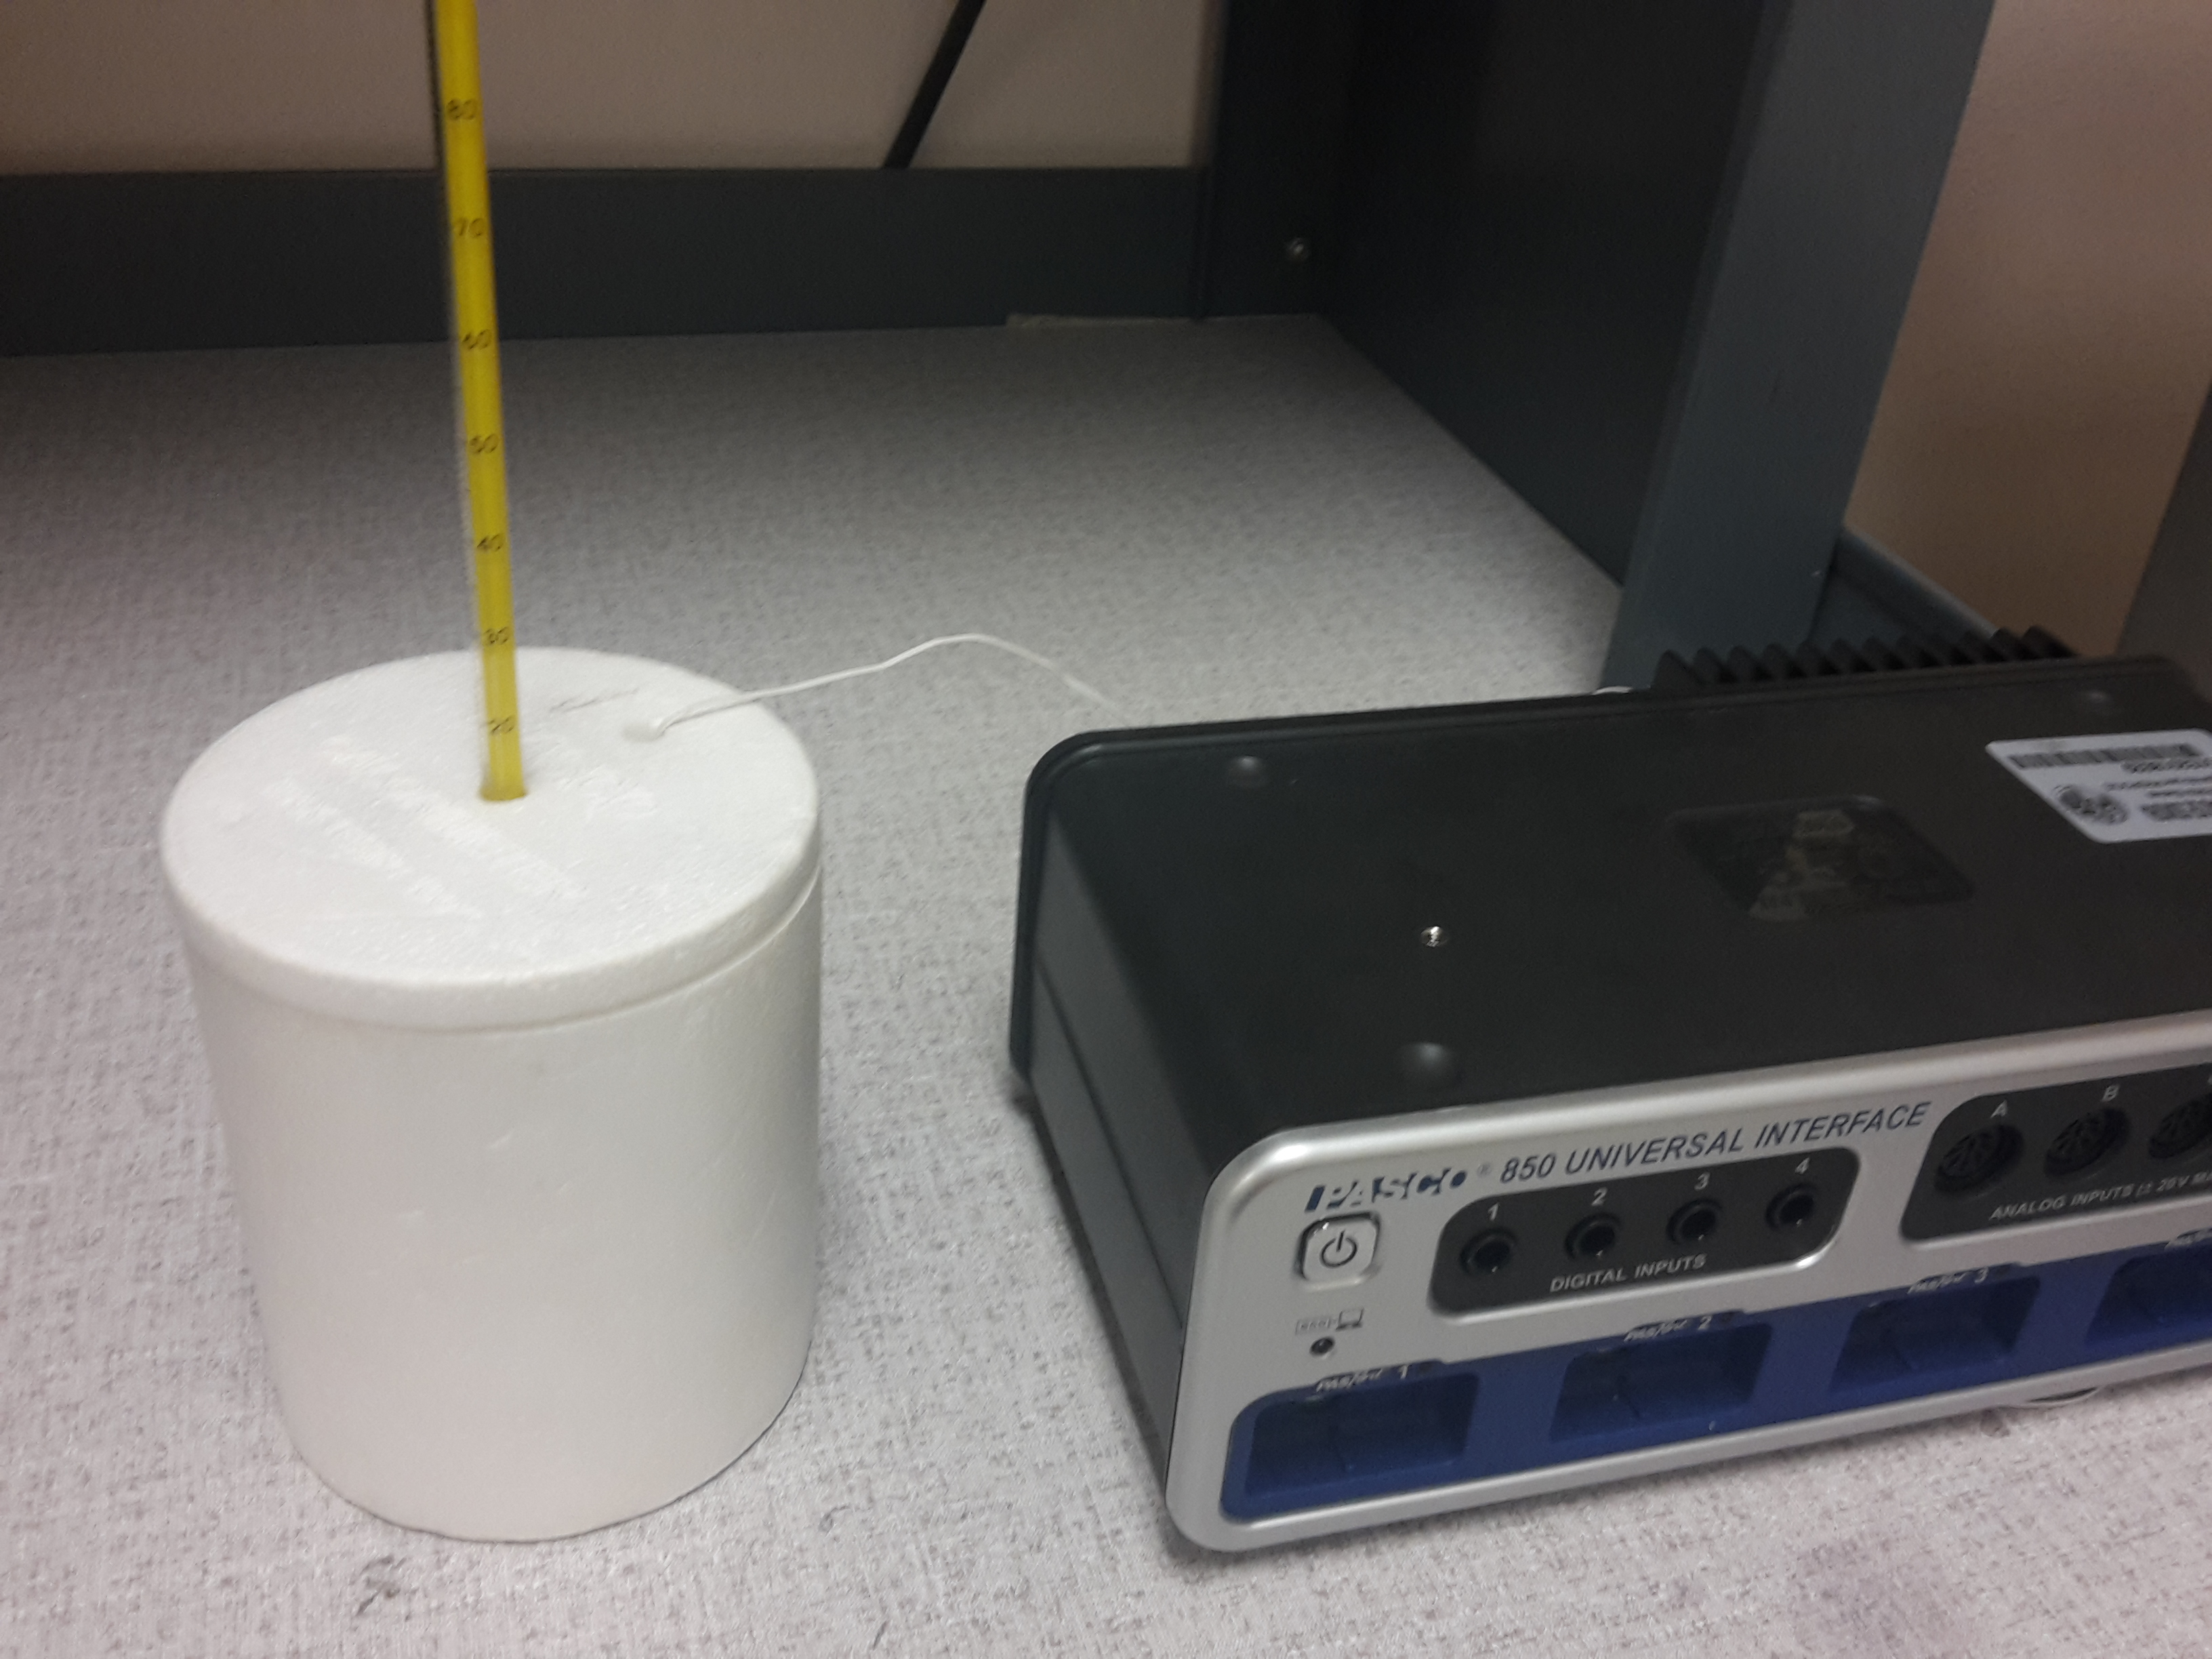
\includegraphics[width=0.25\linewidth]{tempsetup}
\caption{Arreglo de toma de temperatura}
\end{figure}
Al termopar se ajusto a un muestreo de datos de 1Hz. Se empezó a registrar datos de ambos termómetros. Pasados los 5 minutos, se retiro el termómetro de mercurio y se seco. Se volvió a introducir y se siguió la toma de datos. La temperatura de la habitación se tomo durante toda la toma de los datos.

Una vez que se termino de medir la temperatura, se procedió a tomar datos de la presión del laboratorio. Se utilizó  un barómetro PHYWE \cite{barman}, el cual tiene un rango de medición de 0 hPa a 1300 hPa y una exactitud de $\pm$0.5 hPa y una resolución de 0.1 hPa. También se uso un sensor de presión absoluta modelo CI-6532A \cite{bardigi}, el cual tiene un rango de medición de 0 kPa a 700 kPa y una exactitud de $\pm$0.5 kPa y resolución de 0.01 kPa. 
\begin{figure}[H]
\centering
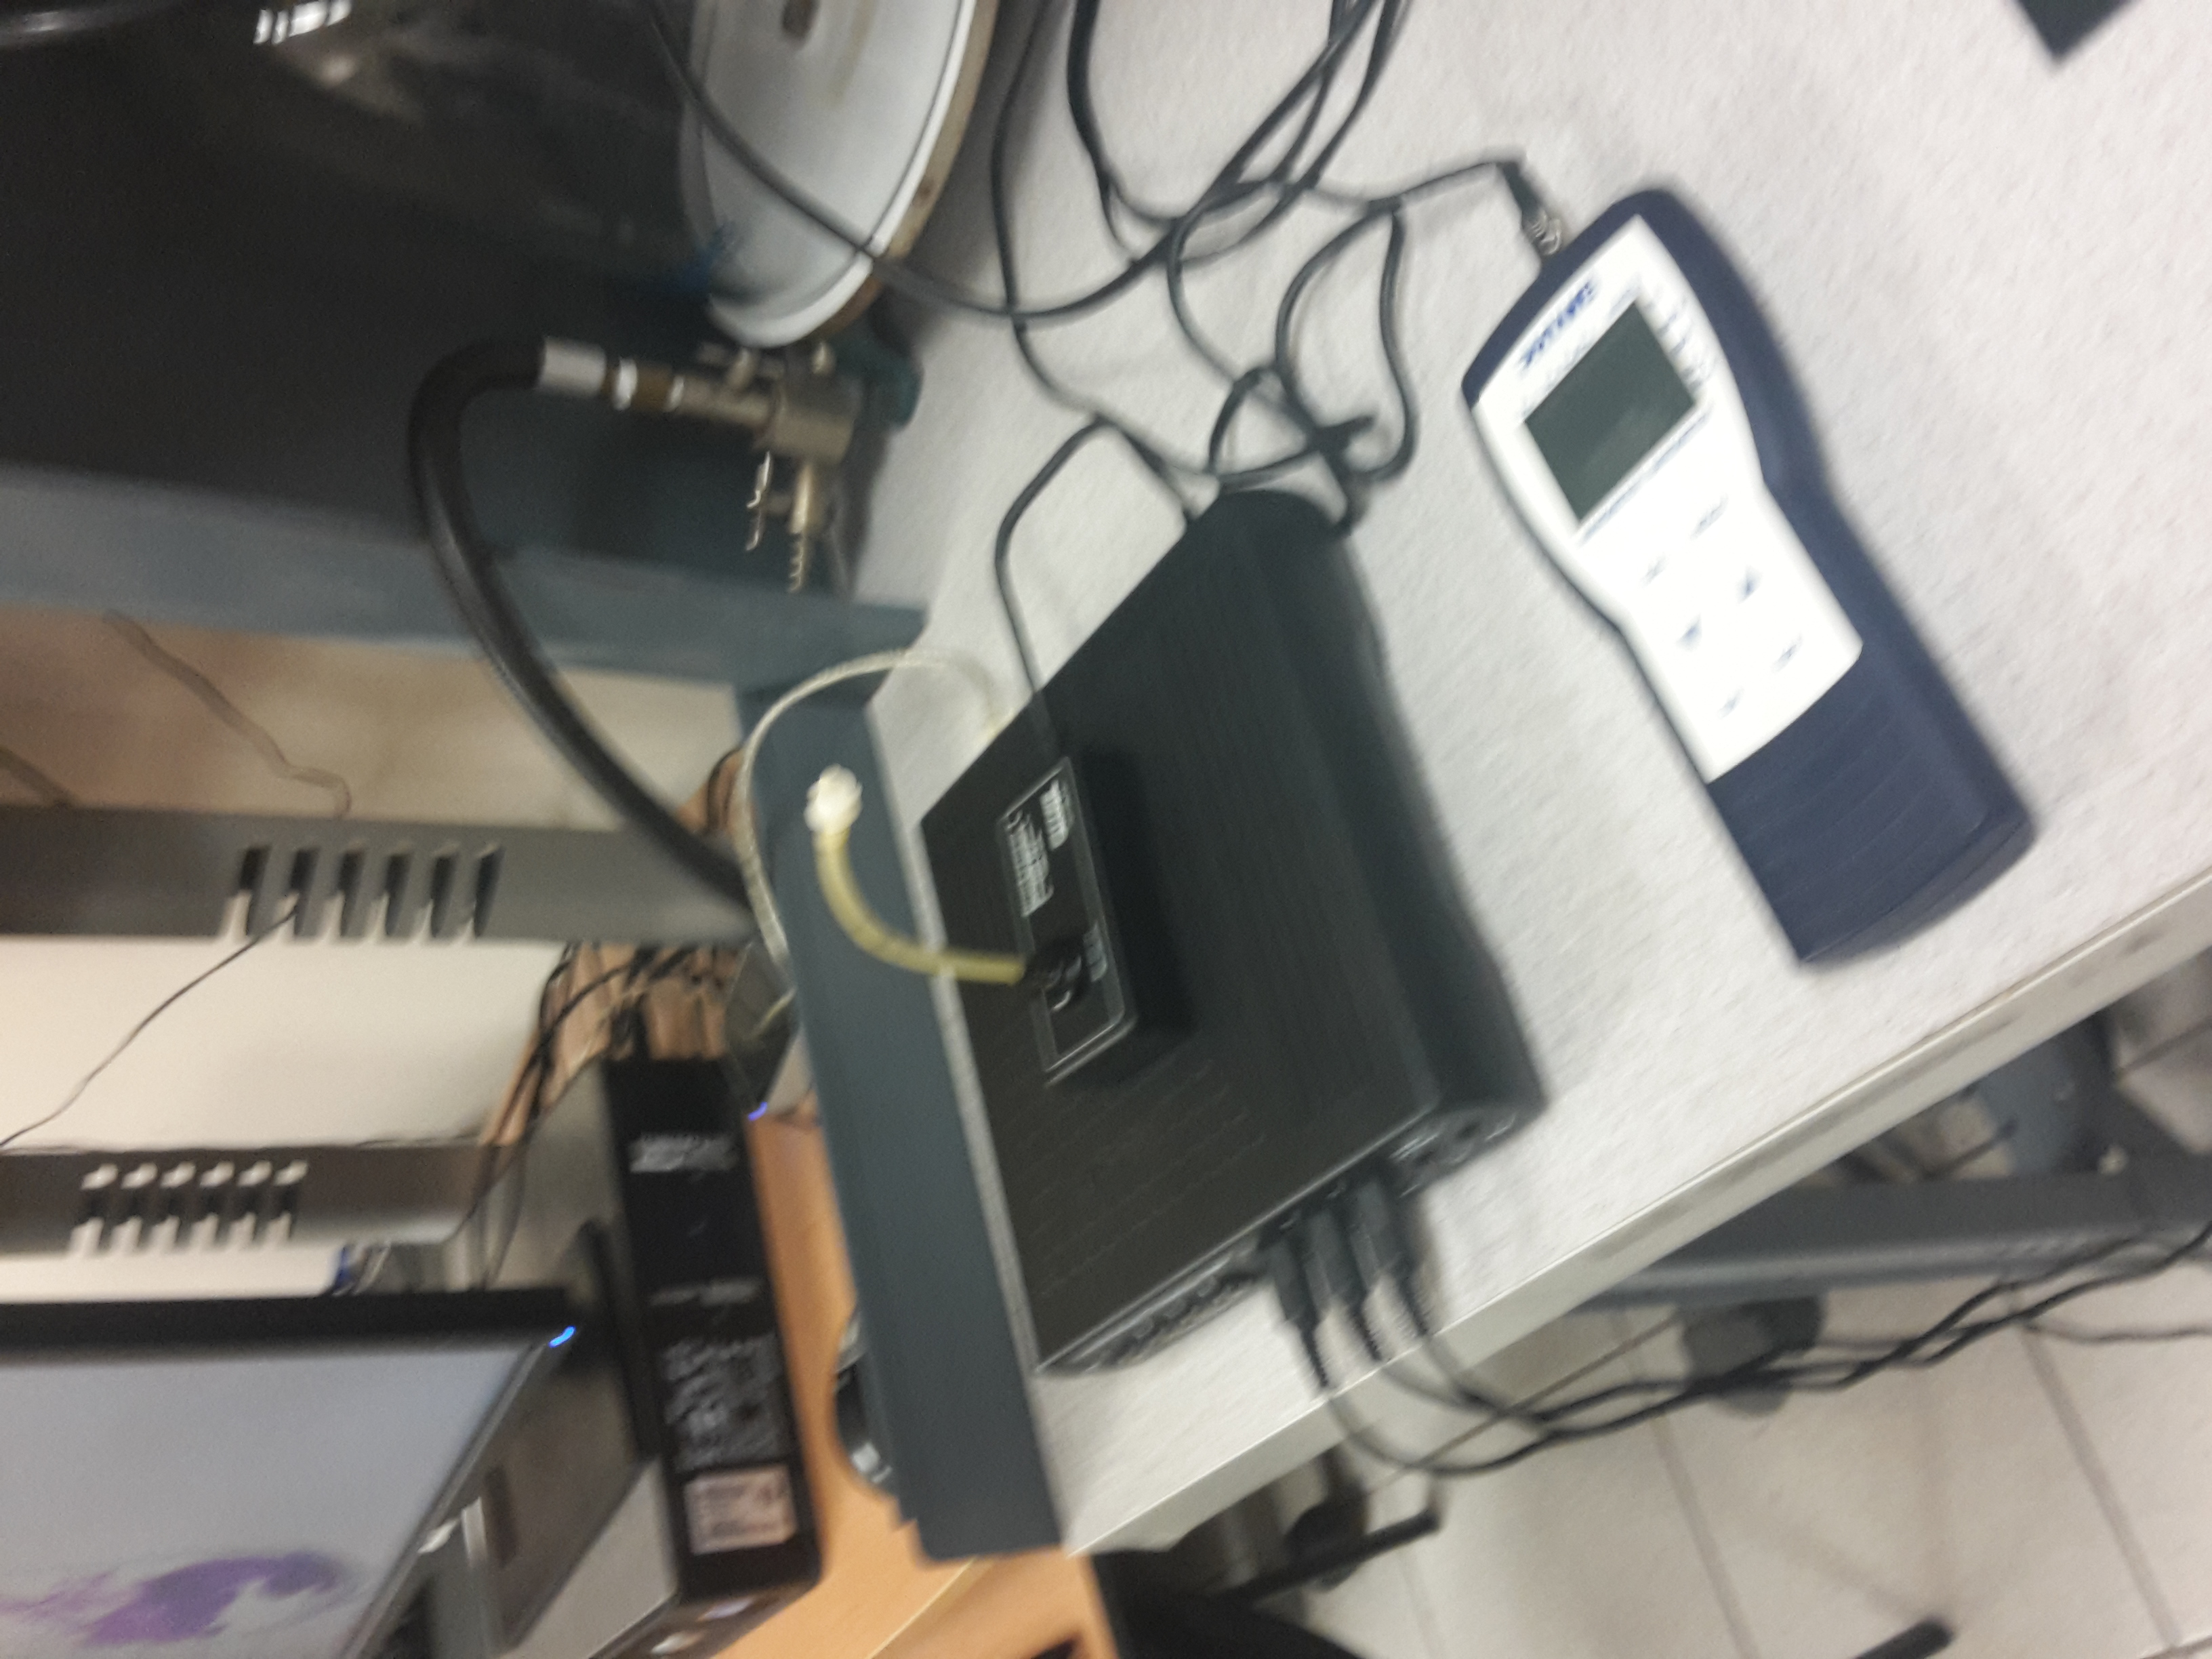
\includegraphics[width=0.25\linewidth]{presetup}
\caption{Arreglo de toma de presión}
\end{figure}
Se registraron datos de la presión de ambos instrumentos y de temperatura por 5 minutos.
\pagebreak
%===================================================================================================
\section{Resultados}
	Los resultados de la medición de la temperatura se pueden observar en la tabla  1. 
\begin{table}[H] 
\centering
\begin{tabular}{|c|c|c|}
\hline
Mercurio(°C) & Termopar(°C) \\\hline
10 $\pm 0.54$ & 10.1 $\pm 0.5$ \\ \hline
10 $\pm 0.54$ & 10.7 $\pm 0.5$\\ \hline
\end{tabular}
\\
Temperatura Ambiente: 21$\pm$0.5°C\\
\caption{Medición de Temperatura}
\end{table}
La incertidumbre proviene de la resolución y de la exactitud que nos proporciona el manual del instrumento.

La incertidumbre por la resolución se calculó mediante el uso de las siguientes expresiones:

Para lectura del termómetro de mercurio:
$$ u(x_i) = \frac{a/2}{\sqrt{6}} = \frac{1/2}{\sqrt{6}} = 0.2041$$
donde a es la resolución. Para el termopar:
$$ u(x_i) = \frac{a/2}{\sqrt{3}} = \frac{0.01/2}{\sqrt{3}} = 0.0029$$
Para agregar la exactitud del instrumento provisto por el manual se realiza:
Para el de mercurio:
$$ \Delta x = \sqrt{u^2+ e^2} = \sqrt{ 0.2041^2+ 0.5^2} = 0.54$$
donde $u$ es el error por resolución y $e$ por exactitud. Para el termopar:
$$ \Delta x = \sqrt{u^2+ e^2} = \sqrt{ 0.0029^2+ 0.5^2} = 0.5$$

En la tabla 2 se muestran los valores de la presión del laboratorio medida por los dos instrumentos.
\begin{table}[H]
\centering
\begin{tabular}{|c|c|}
\hline
Barómetro (mmHg) & Sensor (kPa)  \\\hline
738 $\pm0.5$ & 99.7 $\pm0.5$  \\ \hline
\end{tabular}\\
Temperatura Ambiente: 22$\pm$0.54°C\\
\caption{Medición de Presión}
\end{table}
La incertidumbre proviene de la resolución y de la exactitud que nos proporciona el manual del instrumento.	
Para lectura del PHYWE:
$$ u(x_i) = \frac{a/2}{\sqrt{3}} = \frac{0.1/2}{\sqrt{3}} = 0.0289$$
donde a es la resolución. Para el sensor de presión absoluta modelo CI-6532A:
$$ u(x_i) = \frac{a/2}{\sqrt{3}} = \frac{0.01/2}{\sqrt{3}} = 0.0029$$
Para agregar la exactitud del instrumento provisto por el manual se realiza:
Para el PHYWE:
$$ \Delta x = \sqrt{u^2+ e^2} = \sqrt{ 0.0289^2+ 0.5^2} = 0.5$$
donde $u$ es el error por resolución y $e$ por exactitud. Para el CI-6532A:
$$ \Delta x = \sqrt{u^2+ e^2} = \sqrt{ 0.0029^2+ 0.5^2} = 0.5$$
%===================================================================================================
\section{Discusión}
Lo que se esperaba de esta practica con lo que respecta a la temperatura era obtener un valor cercano a los 10°C lo que cual se logro. En la presión se esperaba una cercana a la presión atmosférica, la cual no se encontró muy lejana. Encontrar las incertidumbres nos permitió identificar que tan buenos son los datos que se midieron.

%===================================================================================================
\section{Conclusiones}
La realización de la medición de temperatura y de la presión se acercaron a la realidad. Las incertidumbres que se calcularon no fueron de gran magnitud. Los pasos que se siguieron considero que no fueron los mejores, pero es una muy buena forma de observar la importancia del instrumento que se utiliza para medir.

\pagebreak
%================================================================================================
\begin{thebibliography}{6}
\bibitem{escala}
	Andres Rico (s.f.) Escalas de Temperatura Recuperado de: \url{ https://tublockupn.wordpress.com/escalas-de-temperatura/}

\bibitem{press}
	Ángel Franco García (s.f.) \textit{Concepto de presión} Recuperado de: \url{http://www.sc.ehu.es/sbweb/fisica_/fluidos/estatica/introduccion/Introduccion.html}
	
\bibitem{termoHg}
	Brannan: \textit{Thermometers and instrumentation scientific catalogue.} \url{http://www.brannan.co.uk}

\bibitem{termopasco}
	\textit{Quad Temperature Sensor PS}-2143.  \url{http://www.pasco.com}

\bibitem{barman}
	\textit{PHYWE: Hand-held measuring instrument pressure (barometer/
manometer).} \url{http://www.phywe-es.com/883/Inicio.htm.}

\bibitem{bardigi}
\textit{Instruction Sheet for the PASCO Model CI-6532A.} \url{http://www.pasco.com.}

\bibitem{acu}
Acu\~na, H. (2015). \textit{Manual de Guías de Experiencias en el Laboratorio de Termodinámica Clásica}.

\end{thebibliography}
%================================================================================================

\end{document}

